\documentclass[11pt,a4paper,titlepage, ngerman]{article}

\usepackage[utf8]{inputenc}	% Diese Pakete sind
\usepackage[T1]{fontenc}		% für die Verwendung 
\usepackage{ngerman}			% von Umlauten im tex-file
\usepackage{lmodern}			% Schriftart, die am Bildschirm besser lesbar ist
\usepackage{graphicx}			% Zum Einbinden von Formeln
\usepackage{url}					% Zur Darstellung von Webadressen
\usepackage{siunitx}
\usepackage{amsmath}			% für equation*
\usepackage{subcaption}

\begin{document}
	\setlength{\parindent}{0em} 
	
	\begin{titlepage}
		\centering
		{\scshape\LARGE Versuchsbericht zu \par}
		\vspace{1cm}
		{\scshape\huge S1 -- Was ist Experimentieren?\par}
		\vspace{2.5cm}
		{\LARGE Gruppe 10 Mi\par}
		\vspace{0.5cm}
		{\large Alex Oster (E-Mail: a\_oste16@uni--muenster.de) \par}
		{\large Jonathan Sigrist (E-Mail: j\_sigr01@uni--muenster.de ) \par}
		\vfill
		durchgeführt am 18.10.2017\par
		betreut von\par
		{\large Dr. Anke \textsc{Schmidt}}
		
		\vfill
		
		{\large \today\par}
	\end{titlepage}
		
	\tableofcontents
	
	\newpage
	
	\section{Einleitung}
		\label{Einleitung}
		
		In diesem Bericht, zur ersten experimentellen Übung, beschäftigen wir uns mit der Frage, was genau man unter dem Begriff \glqq Experimentieren\grqq\ verstehen sollte. Dazu betrachten wir zunächst folgende Fragen:
	
		\begin{enumerate}
			
			\item Was ist mit \glqq Messgröße\grqq\ gemeint?
			\item Warum führt man Experimente in der Naturwissenschaft durch? und
			\item Weshalb kann der \glqq wahre Wert\grqq\ einer Messgröße niemals bestimmt werden?
			
		\end{enumerate}
			
			Zur Beantwortung dieser Fragen, wenden wir uns nun drei einfachen Versuchen zu, welche die Bedeutung von Messungenauigkeiten durch unterschiedliche Messverfahren verdeutlichen sollen. In dem ersten Versuch haben wir die Leerlaufspannung einer 9V-Batterie gemessen, in dem zweiten Versuch die Länge eines \glqq STABILO point 88\grqq\ Stiftes und in dem dritten Versuch dann die Zeit, die Kugeln verschiedener Masse zum Herunterrollen einer schiefen Ebene benötigen.\\
		
			Die Auswertungen dieser Versuche werden wir dann in \textbf{(\ref{Diskussion} Diskussion)} mit den obigen Fragen verknüpfen und damit den Begriff \glqq Experimentieren\grqq {} erklären.
	
	\newpage
	\section{Durchführung}
		\label{Durchführung}
		
		\subsection{Versuch 1: Leerlaufspannung}
			\label{2.1}
			
			In diesem Versuch geht es um die Messung der Leerlaufspannung einer \SI{9}{\V}-Batterie mit Hilfe eines digitalen Multimeters. Wir fragen uns zunächst, welche Werte für die Leerlaufspannung $U_0$ realistisch wirken und stellen eine Hypothese bzw. Erwartungsbereich auf.
			
			\subsubsection{Vorwissen und Aufstellen einer Hypothese}
				\label{2.1.1}
				
				Da es sich um eine \SI{9}{\V}-Batterie handelt und da keine negativen Werte für $U_0$ vorliegen können, schließen wir darauf, dass der Wert für die Leerlaufspannung sich mindestens im Bereich von \SIrange{0}{9}{\V} befinden sollte.
				Das, am Boden der Batterie, gegebene Mindesthaltbarkeitsdatum (\glqq 2020\grqq) wurde noch nicht überschritten, weswegen bis dahin die \SI{9}{\V} garantiert sein sollten. Also folgern wir, dass die Batterie, im unbenutzten Falle, auch mehr als \SI{9}{\V} Leerlaufspannung besitzen könnte.
				Deswegen haben wir unseren Erwartungsbereich von \SIrange{0}{9}{\V} auf \SIrange{0}{10}{\V} erweitert(\ref{fig:spannung}, links).
				
				\begin{figure}	
					\begin{subfigure}{0.45\textwidth}
						\centering
						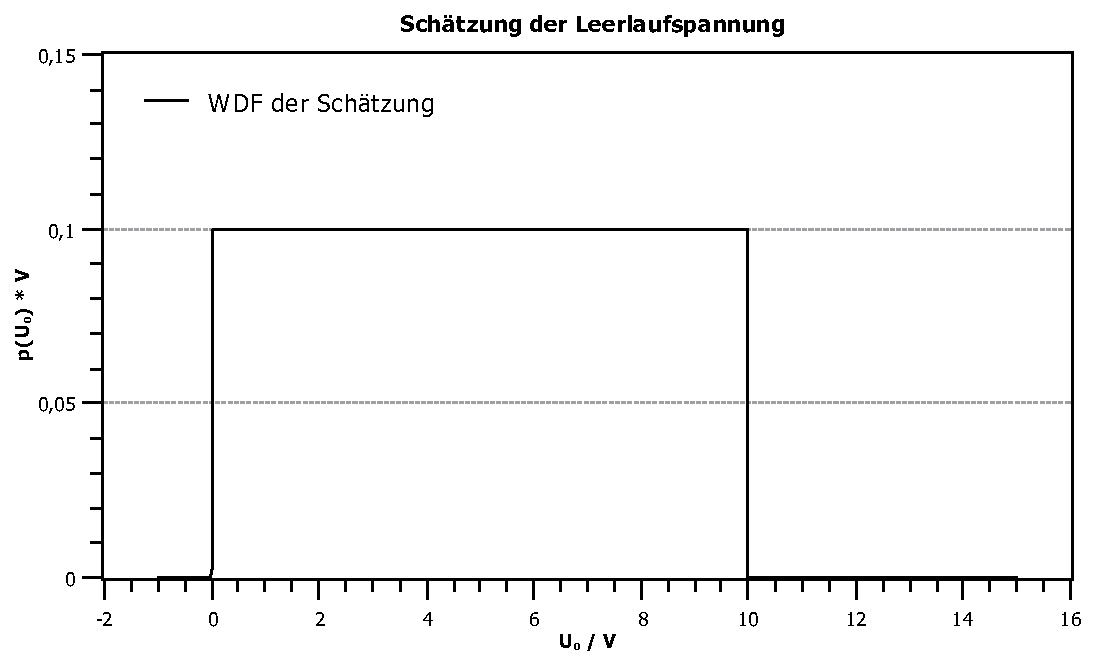
\includegraphics[scale=0.3]{Spannungsschaetzung.pdf}
					\end{subfigure}
					\begin{subfigure}{0.45\textwidth}
						\centering
						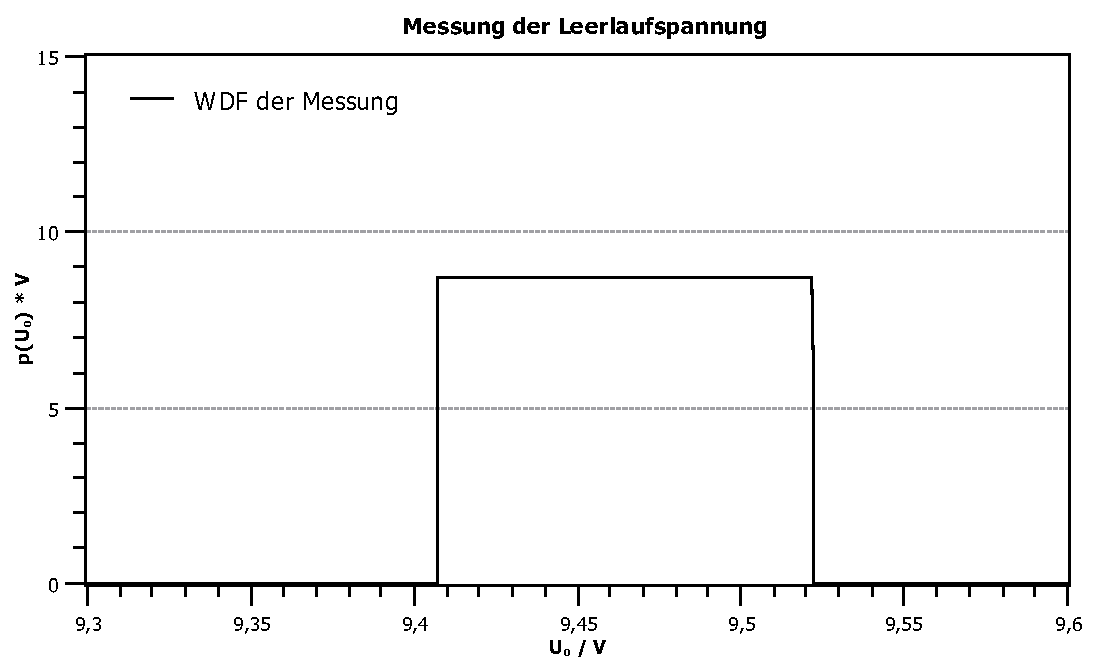
\includegraphics[scale=0.3]{Spannungsmessung.pdf}
					\end{subfigure}	
					\caption{Schätzung und Messung der Leerlaufspannung.}
					\label{fig:spannung}
				\end{figure}
			
			\subsubsection{Messwerte, Ungenauigkeitsbetrachtung und Ergebnis}
				\label{2.1.2}
				
				Zur Durchführung der Messung haben wir das Multimeter erst auf den zu erwartenden Messbereich von ungefähr \SI{10}{\V} kalibriert und dann mit einfachen Kabeln an die \SI{9}{\V}-Batterie angeschlossen. \\			
				Die, von dem Gerät, gemessenen Werte schwankten zwischen \SI{9,46}{\V} und \SI{9,47}{\V}.
				Da das Messgerät rundet betrachten wir hierbei Werte von \SIrange{9,455}{9,475}{\V}.
				Zudem besitzt das Messgerät eine Ungenauigkeit von $0.5\%$ des angegebenen Wertes, weswegen der eigentliche Wert im Bereich von \SIrange{9,407}{9,522}{\V} liegt(\ref{fig:spannung}, rechts).
			\newpage
				\begin{flushleft}
					Somit ergibt sich:\\
					\vspace{0.5cm}
					$U_0 \in [\SI{9.407}{\V},\SI{9.522}{\V}]$\\
					$a = \SI{0.115}{\V}$ \\
					$\sigma = \SI{0,0332}{\V}$ \\
					\vspace{0.5cm}
					wir erhalten einen den Erwartungen entsprechenden Wert von: \\ 
					\vspace{0.5cm}
					$U_0 = (9,4645 \pm 0,0332)\si{\V}$\\ 
				\end{flushleft}
	
		\vspace{2cm}
		\subsection{Versuch 2: Längenmessung}
			\label{2.2}
			
			Der zweite Versuch beschäftigt sich mit der Messung der Länge eines Stiftes. Und auch hier fragen wir uns zuerst, welche Werte für die Länge des Stiftes in Frage kommen.
		
			\subsubsection{Schätzung}
				\label{2.2.1}
				
				Die Stiftlänge haben wir über die Spannbreite von Daumen und Zeigefinger in ein Intervall von \SIrange{15}{20}{\cm} abgeschätzt(\ref{fig:laenge}, links).
				
				\begin{figure}	
					\begin{subfigure}{0.45\textwidth}
						\centering
						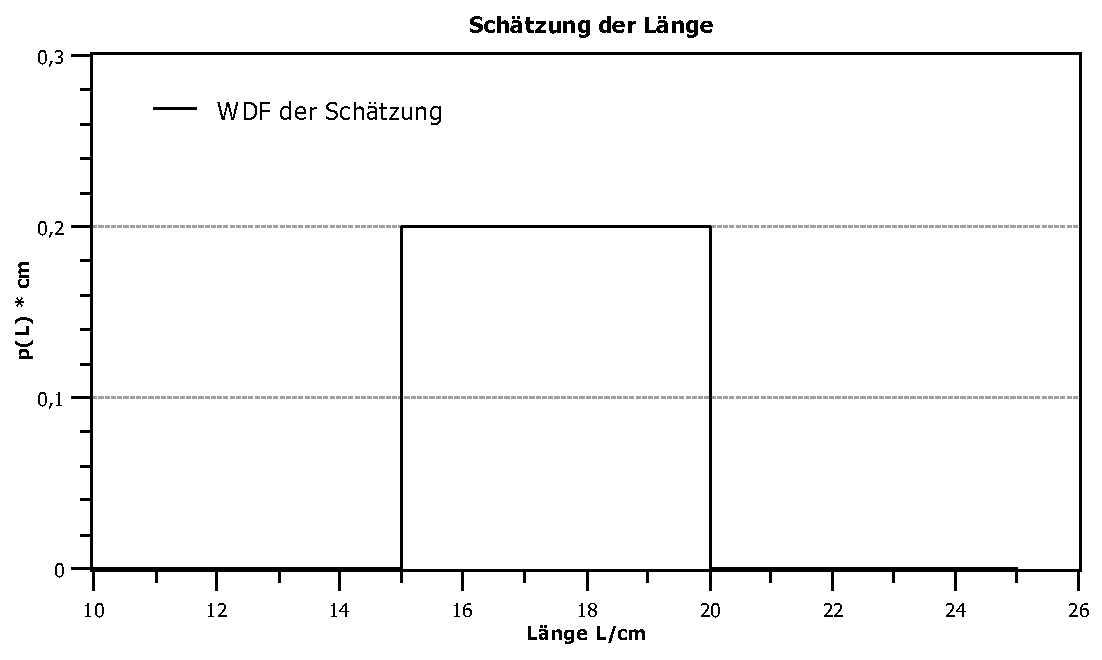
\includegraphics[scale=0.3]{Laengenschaetzung.pdf}
					\end{subfigure}
					\begin{subfigure}{0.45\textwidth}
						\centering
						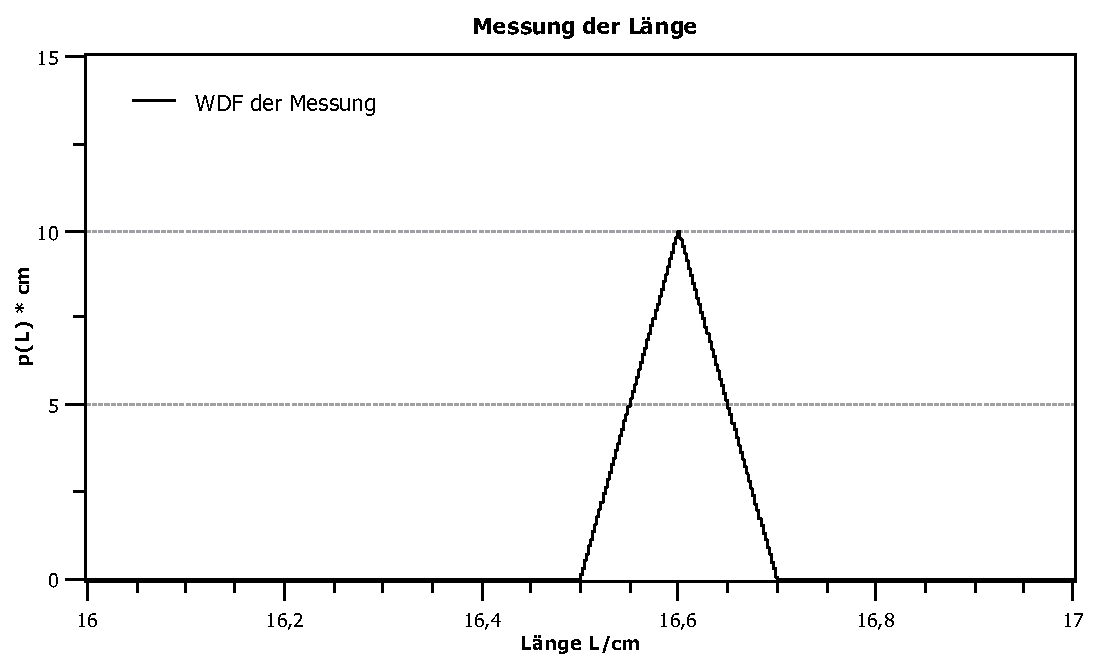
\includegraphics[scale=0.3]{Laengenmessung.pdf}
					\end{subfigure}	
					\caption{Schätzung und Messung.}
					\label{fig:laenge}
				\end{figure}
				
			\subsubsection{Messung}
				\label{2.2.2}
				
				Mit Hilfe eines handelsüblichen Maßbandes haben wir die Messung durchgeführt. Sie ergab eine Länge von ca. \SI{16,6}{\cm} von beiden Seiten(\ref{fig:laenge}, rechts). Die Unsicherheit des Maßbandes wurde hierbei nicht betrachtet, da kein realistischer Wert dafür gegeben war (\SI{6}{\cm} Ungenauigkeit auf \SI{2}{\m}).
			
		\newpage
		\subsection{Versuch 3: Schiefe Ebene}
			\label{2.3}
			
			In dem dritten Versuch messen wir die Zeit, die zwei Kugeln aus verschiedenem Material für das Herunterrollen einer schiefen Ebene benötigen, um die Frage zu beantworten, ob die Masse einer Kugel zu ihrer Geschwindigkeit beim Herunterrollen beiträgt.	
					
			\subsubsection{Hypothese}
				\label{2.3.1}
				
				Hierfür haben wir die Hypothese aufgestellt, dass schwere Kugeln schneller als Leichtere, gleichen Volumens, die schiefe Ebene herunterrollen. Also: 
				\begin{equation*}
					(m_1 < m_2 \wedge V_1 = V_2) \Rightarrow v_1 < v_2
				\end{equation*}
					
			\subsubsection{Messung, Beobachtung und Messwerte}
				\label{2.3.2}
				
				Um die Hypothese zu verifizieren bzw. falsifizieren, haben wir eine Holzkugel und eine Metallkugel, mit gleichem Radius, mehrfach eine schiefe Ebene herunterrollen lassen und dabei die Zeit gemessen, die sie dafür gebraucht haben.
				
				Dabei haben wir kleine Ungenauigkeiten, welche u.A. durch den Luftwiderstand und Reibung aufgerufen werden, nicht genauer betrachtet. \\
				
				Diese Messung haben wir 15 mal pro Kugel durchgeführt, sodass der Mittelwert über alle Messungen sich mit jeder neuen Messung nicht merklich geändert hat: \SI{1.713}{\s} für die Metallkugel und \SI{1.791}{\s} für die Holzkugel.
				
				
				\begin{figure}		
				\begin{subfigure}{0.45\textwidth}
					\label{HistogrammV3}
					\centering
					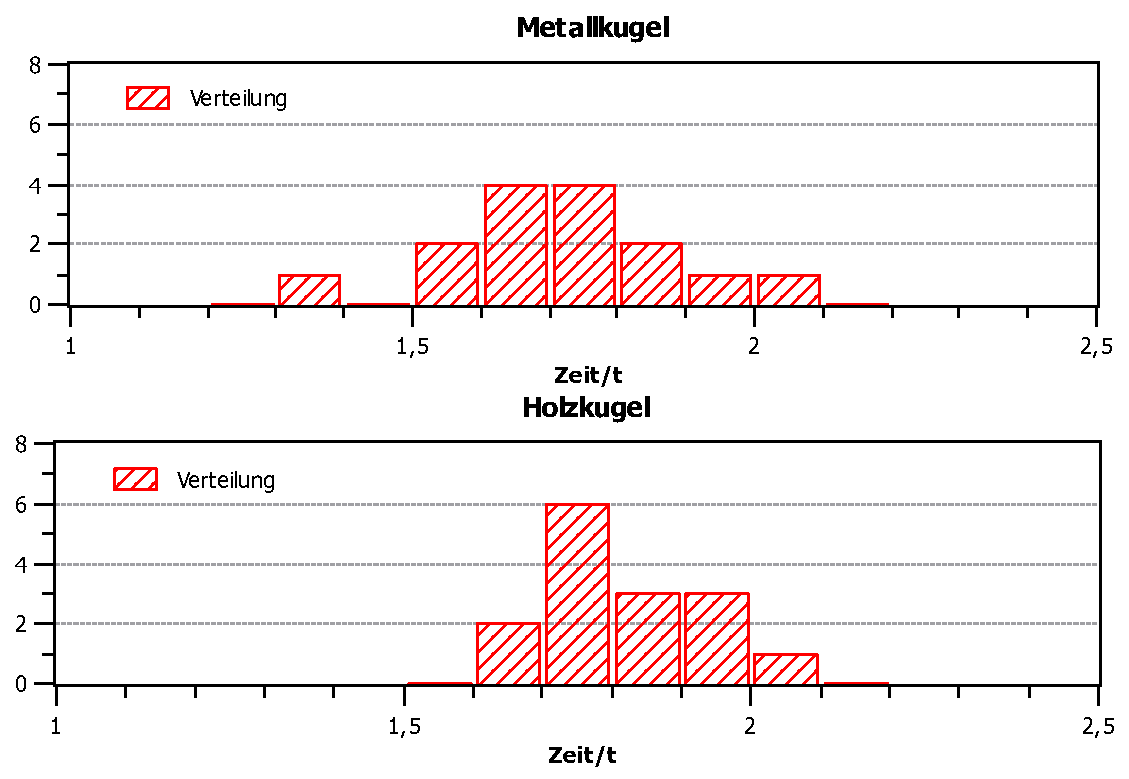
\includegraphics[scale=0.3]{Histogramm.pdf}
					\caption{Verteilung der Messwerte.}
				\end{subfigure}
				\begin{subfigure}{0.45\textwidth}
					\label{MittelwerteV3}
					\centering
					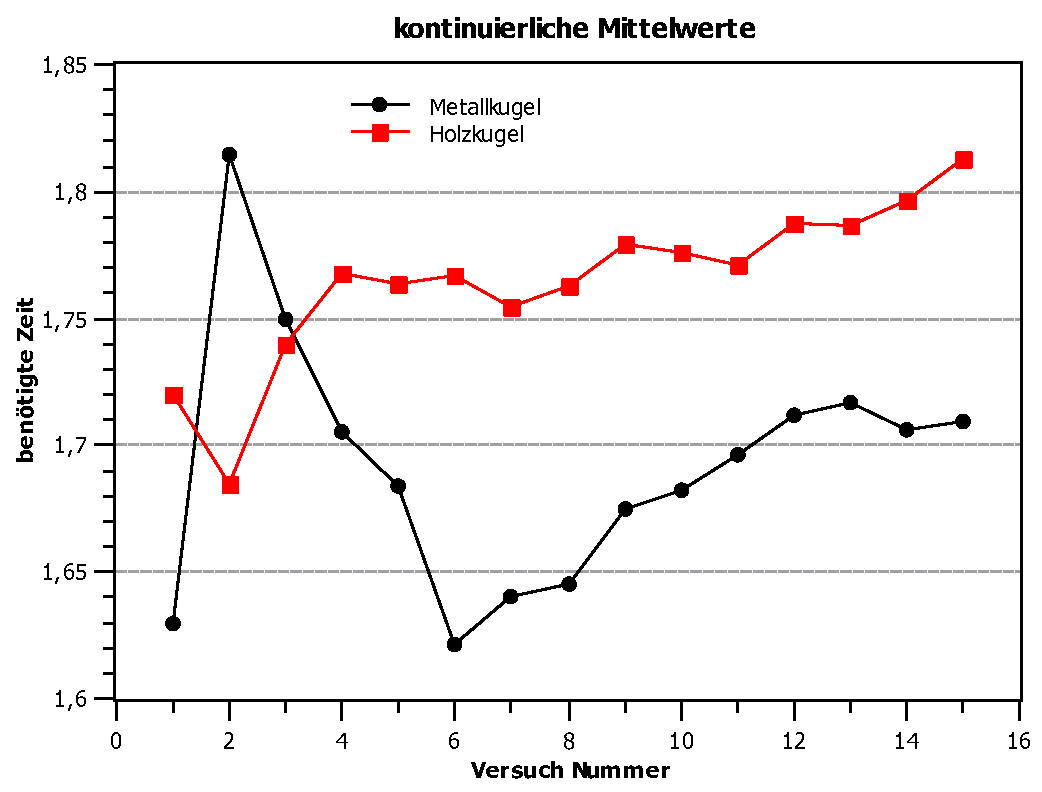
\includegraphics[scale=0.3]{Mittelwerte.pdf}
					\caption{Entwicklung der Mittelwerte.}
				\end{subfigure}	
				\caption{Ergebnisse der Messung.}
				\end{figure}
			
				\begin{table}
					\label{Tab:VerteilungsWerte}
					\centering
					\begin{tabular}{l|SSS}
						\hline
						& {$\mu$} & {$\sigma$} & {$u$} \\ \hline
						Metallkugel & 1,709 & 0,1512 & 0,039\\
						Holzkugel & 1,813 & 0,1035 & 0,0267\\ \hline
					\end{tabular}
					\caption{Mittelwert, Standardabweichung und Standardunsicherheit nach 15 Messungen.}
				\end{table}
		
				Die Werte für Standardabweichungen und Mittelwerte nach 15 Messungen sind in Tabelle 1 dargestellt\footnote{Die Tabelle mit allen einzelnen Messungen, sowie den errechneten Wahrscheinlichkeiten findet sich im Anhang.}.
				
				\newpage
								
				Trotz 15 Messungen hat der Mittelwert für die Holzkugel sich noch um ca. \SI{0.02}{s} vom vorherigen Mittelwert unterschieden. Das könnte an ungenauer Zeitmessung gelegen haben, weswegen weitere Messungen mit Sicherheit ein genaueres Ergebnis geliefert hätten. \\

				Außerdem haben wir zudem noch das zeitgleiche Herunterrollen beider Kugeln betrachtet und festgestellt, dass wenn die Holzkugel vorne ist, immer beide Kugeln gleichzeitig unten ankommen. Ist jedoch die Metallkugel vorne, so kommt sie vor der Holzkugel an.	
				
			\subsubsection{Schlussfolgerung}
				\label{2.3.3}
				
				Der direkte Vergleich der Messwerte und die Beobachtung für zwei zeitgleich rollende Kugeln deuten darauf hin, dass die Hypothese stimmt.
				Das kann durch die wirkende Gravitationskraft und das Trägheitsmoment erklärt werden, welche bei einer schiefen Ebene auf einen Körper ebenfalls von der Masse der Körper abhängen.
				
	\newpage
	\section{Diskussion}	
		\label{Diskussion}
		
		Betrachten wir nun die Fragen aus \textbf{(\ref{Einleitung} Einleitung)}: \\
		
		\begin{enumerate}
			\item \textit{Was ist mit \glqq Messgröße\grqq\ gemeint?} 
				\vspace{0.2cm}\\
				Eine Messgröße ist eine zu messende Größe bzw. das, was gemessen wird.
				Also ein Wert, der nicht genau bekannt ist und deshalb durch Messungen bestimmt werden soll.
				In \ref{2.1} war es die Leerlaufspannung $U_0$, in \ref{2.2} war es die Länge des Stiftes und in \ref{2.3} die Zeit, welche die Kugeln zum Herunterrollen benötigten.
				Messgrößen bieten uns die Möglichkeit, verschiedene Werte im selben Maß zu betrachten, um damit einzuordnen welche Werte größer, kleiner oder realistischer sind, wenn man sie mit dem Erwartungswert vergleicht. \\
				
			\item \textit{Warum führt man Experimente in der Naturwissenschaft durch?}
				\vspace{0.2cm}\\
				Das Ziel von Naturwissenschaften war es schon immer die Vorgänge der Natur zu erklären und Fragen zu beantworten. \\
				Oft wurden und werden Experimente genutzt um Theorien und Hypothesen zu überprüfen. In unserem Falle, waren es Vermutungen, die wir durch kleine Versuche verifiziert haben.
				
				Viele Sachverhalte werden jedoch erst durch in Experimenten gemachten Beobachtungen erkannt.
				Experimente tragen also auch aktiv an der Entdeckung von neuen Gesetzmäßigkeiten bei.\\
				 
			\item \textit{Weshalb kann der \glqq wahre Wert\grqq\ einer Messgröße niemals bestimmt werden?}
				\vspace{0.2cm}\\
				Nein, der wahre Wert einer Messgröße kann nicht bestimmt werden. Unsere Versuche zeigen bereits, dass für die verschiedenen Messgrößen nur Erwartungswerte gefunden werden können, welche meistens ein \glqq breites Intervall\grqq\ aufgrund von Ungenauigkeiten beschreiben.
				Auch Seiteneffekte wie z. B. Reibung müssen für einen möglichst genauen Wert betrachtet werden, was das Finden eines \glqq wahren Werts\grqq\ durch Experimente zusätzlich erschwert.
				
				Letzentlich kann ein Wert selbst bei sehr vielen Messungen aufgrund statistischer und systematischer Unsicherheiten nie auf einen \glqq wahren Wert\grqq\ reduziert werden.\\
				
		\end{enumerate}
		\newpage
		Also was genau sollte man unter dem Begriff \glqq Experimentieren\grqq\ verstehen? \\
		
		\glqq Experimentieren\grqq\ ist, wenn man unter kontrollierten Umgebungen eine Hypothese durch Messungen auf ihre Richtigkeit überprüft.
		Hierbei ist das Ziel jedoch nicht die Bestimmung eines \glqq wahren Werts\grqq\, sondern der eines Erwartungswerts, da ein solcher sich in der Regel bestimmen lässt.
	
		Die Hypothese kann zum Beispiel vorherige Beobachtungen in einen größeren Zusammenhang stellen oder neue Gesetzmäßigkeiten voraussagen, die nun durch das Experiment belegt werden sollen.
		
		\newpage
	\section{Anhang}
		\label{Anhang}
		Abbildungen 4 und 5 auf den nächsten Seiten
		\begin{figure}
			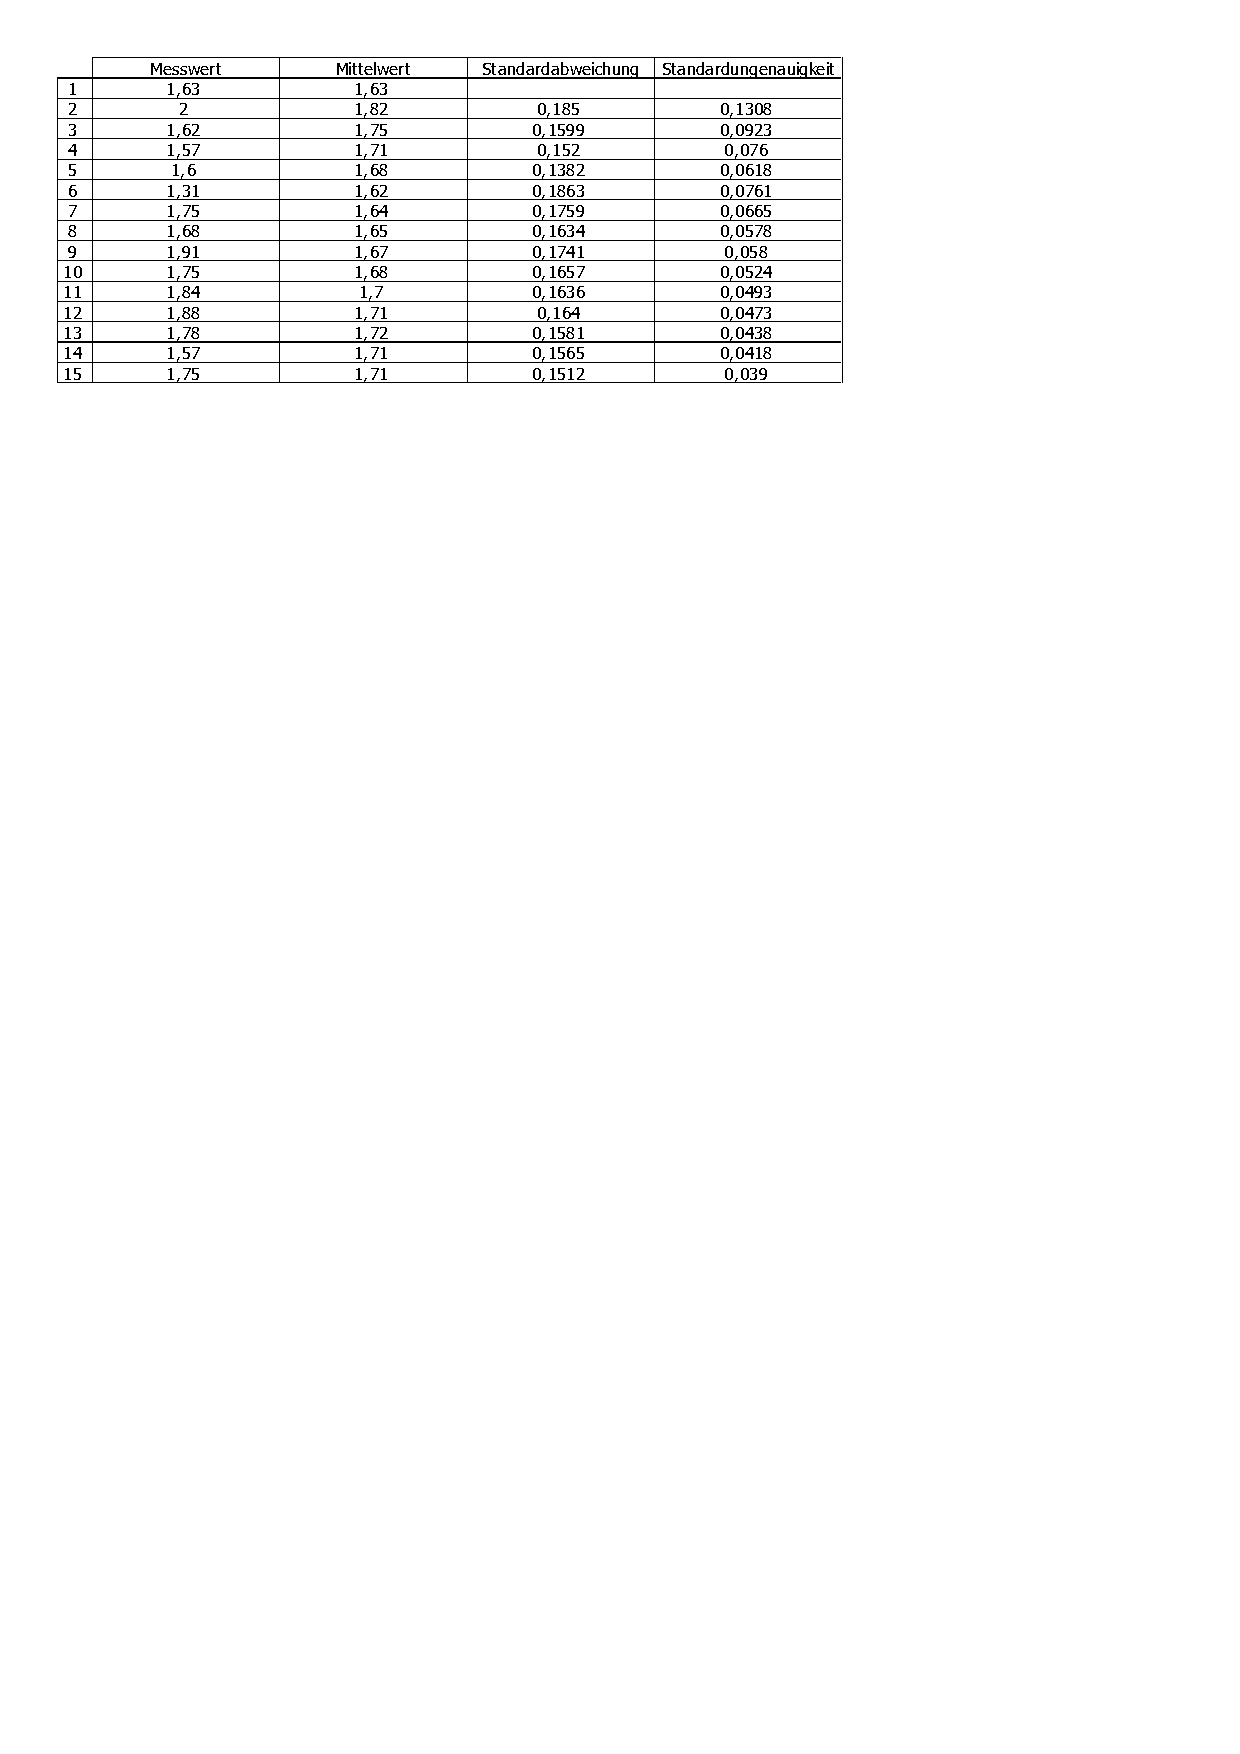
\includegraphics[scale=0.68]{Metallkugel.pdf}
			\caption{Messwerte der Metallkugel.}
		\end{figure}
		\begin{figure}
			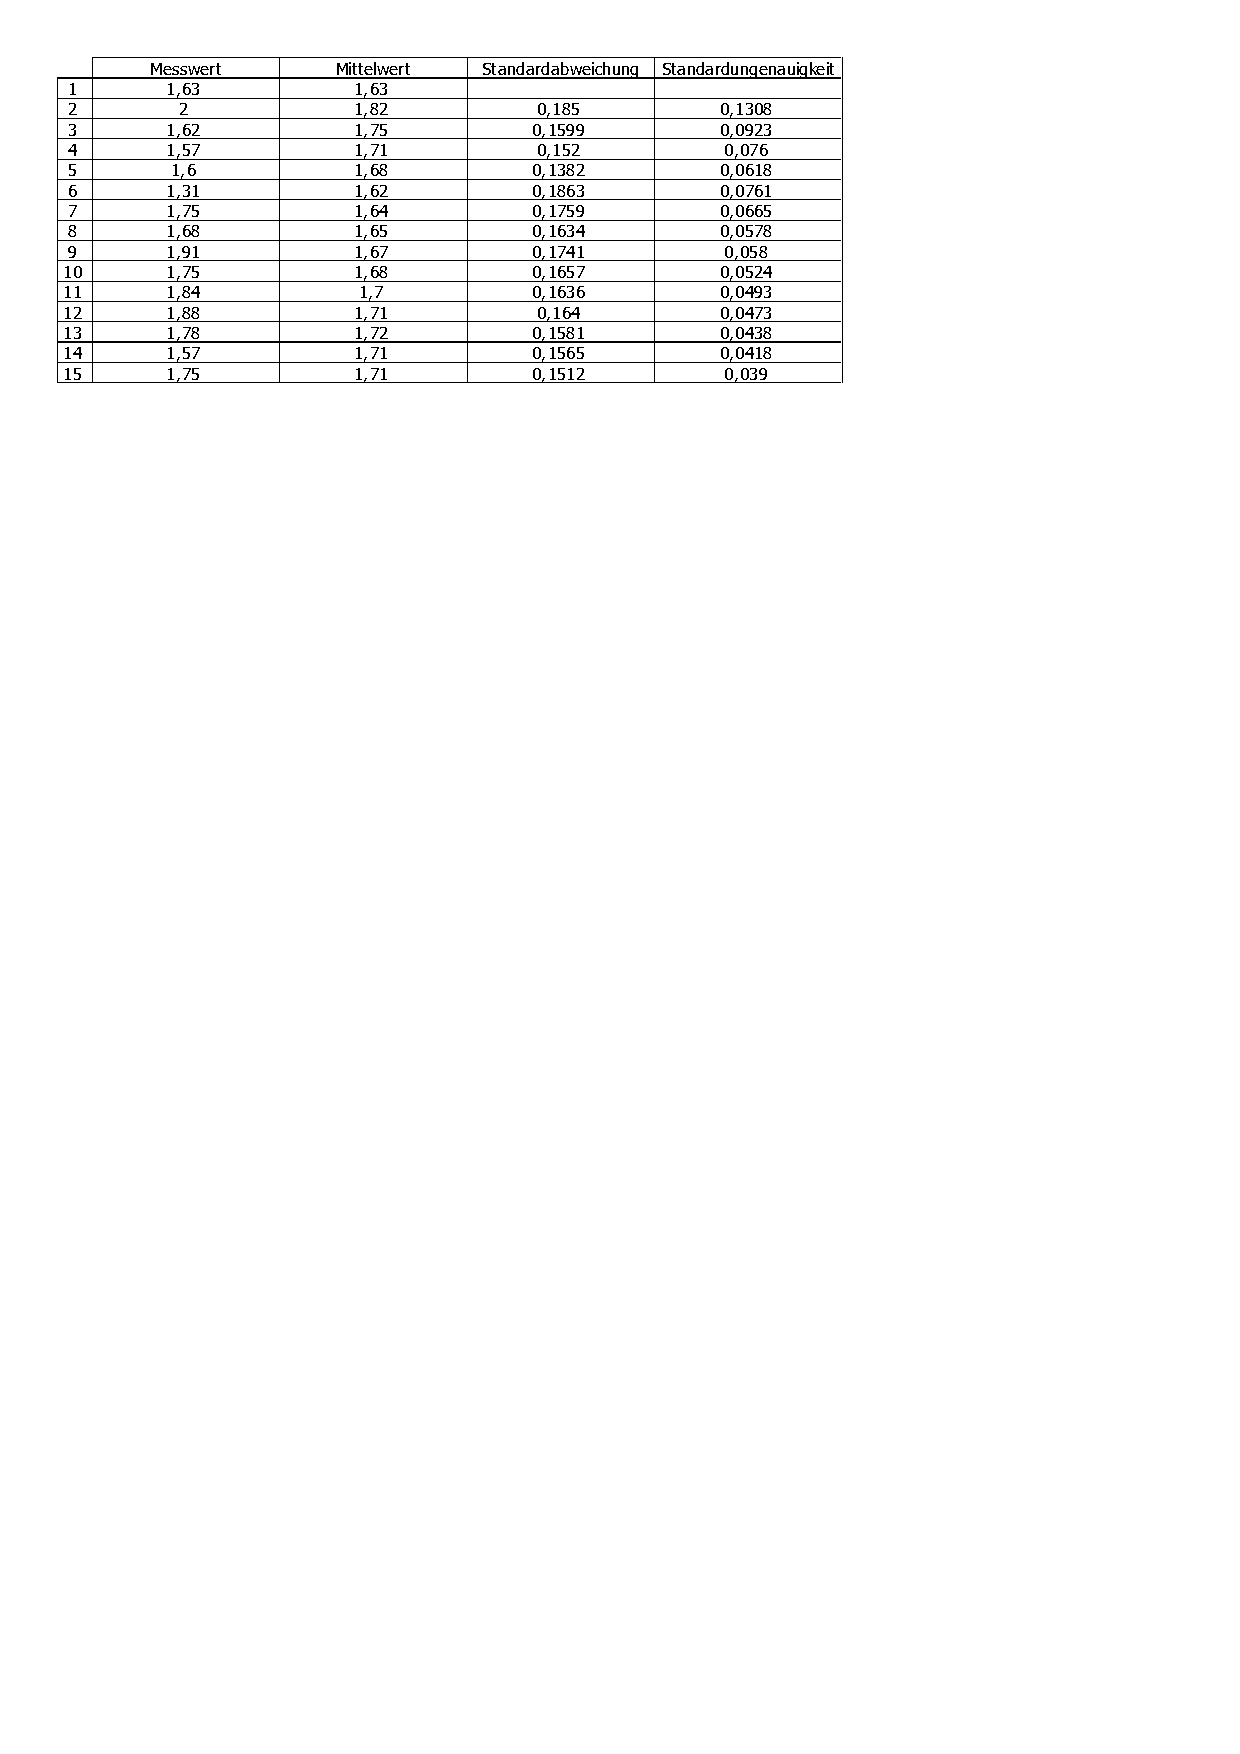
\includegraphics[scale=0.68]{Metallkugel.pdf}
			\caption{Messwerte der Holzkugel.}
		\end{figure}
\end{document} 